\documentclass[11pt,a4paper]{article}
\usepackage[margin=2.2cm]{geometry}
\usepackage{graphicx}
\usepackage{hyperref}
\usepackage{enumitem}
\usepackage{titlesec}
\usepackage{parskip}
\usepackage[T1]{fontenc}
\usepackage{lmodern}

\titlespacing*{\section}{0pt}{10pt}{4pt}
\titlespacing*{\subsection}{0pt}{7pt}{2pt}

\title{\textbf{Synthesizing Robust Adversarial Examples\\via Expectation over Transformations}\\[4pt]
\large Project Summary}
\author{AI Security --- Team 6}
\date{}

\begin{document}
\maketitle
\vspace{-8pt}
\hrule
\vspace{6pt}

% ─────────────────────────────────────────────────────────────────────────────
\section{Objective}

The goal of this project was to reproduce the main result of Athalye et al.\ (2017).
We wanted to modify the texture of a 3D object --- a sea turtle mesh --- in such a way
that an image classifier (InceptionV3, pretrained on ImageNet) consistently predicts
the wrong class regardless of the viewing angle.
In our experiments the target class was \textit{rifle} (class~764)
instead of the correct \textit{loggerhead turtle} (class~33).

What makes this harder than a standard adversarial attack is that the modified texture
must fool the classifier from \textbf{every angle}, with any background colour,
and under varying lighting --- not just from one fixed viewpoint.

% ─────────────────────────────────────────────────────────────────────────────
\section{Core Idea: Expectation over Transformations}

The key technique is called \textbf{Expectation over Transformations (EOT)}.
Instead of optimising the perturbation for a single image,
at every optimisation step we sample many random transformations
(rotations, crops, colour changes) and average the gradient over all of them.
This forces the perturbation to work across the whole distribution of
possible views, not just one specific one.

% ─────────────────────────────────────────────────────────────────────────────
\section{2D Pipeline}

The 2D pipeline serves as a simpler baseline that works directly on images.

\textbf{Input.} A single image (in our case the turtle texture photograph).

\textbf{What we optimise.} A small additive noise pattern (perturbation)
added on top of the image pixels, constrained so that it is nearly invisible
to the human eye.

\textbf{Random transformations.} At each step we apply random combinations of:
\begin{itemize}[noitemsep,topsep=2pt]
  \item random rotation ($\pm30^\circ$), scaling and small translation,
  \item random brightness and contrast shifts,
  \item small Gaussian pixel noise.
\end{itemize}
These are all differentiable operations, so the gradient of the loss
flows back through them to the perturbation.

\textbf{Optimisation.} We run 200 steps of Projected Gradient Descent (PGD).
At each step we compute how wrong the classifier is about the target class,
averaged over 20 randomly transformed copies of the image,
and nudge the perturbation in the direction that makes the classifier
more likely to predict the target class.
After each step the perturbation is clipped to stay within the allowed budget.

% ─────────────────────────────────────────────────────────────────────────────
\section{3D Pipeline}

The 3D pipeline extends the idea to a full 3D object.

\textbf{What we optimise.} Instead of perturbing pixels,
we optimise the \textbf{UV texture map} of the mesh ---
the image that is ``painted'' onto the surface of the 3D model.

\textbf{How gradients reach the texture.}
The render pipeline works as follows:
the texture is sampled at the UV coordinates of each visible pixel
(using bilinear interpolation, which is differentiable),
the result is passed to the classifier,
and the gradient of the loss is propagated back through the classifier
and through the texture sampling step all the way to the texture map.
The triangle rasterisation step (deciding which pixels belong to which triangle)
is not differentiable, but this is not a problem --- we only need
gradients to reach the texture values.

\textbf{Random transformations.} At each step we sample random camera poses:
\begin{itemize}[noitemsep,topsep=2pt]
  \item fully random 3D rotation (any direction),
  \item random camera distance and small lateral shift,
  \item random background colour.
\end{itemize}

\textbf{Optimisation.} We run 500 steps of PGD with 40 random viewpoints per step.
After each step the texture values are clipped to the valid colour range $[0, 1]$.

\textbf{Implementation.}
We used InceptionV3 (torchvision, frozen weights) as the classifier.
The renderer uses PyTorch3D when available; a pure-NumPy software fallback
is also implemented for environments where PyTorch3D cannot be installed
(gradients are preserved via \texttt{F.grid\_sample}).
The turtle mesh has 36\,924 vertices and 73\,844 triangles
with a $256\times256$ texture map.

% ─────────────────────────────────────────────────────────────────────────────
\section{Results}

Figure~\ref{fig:results} shows six random viewpoints of the turtle mesh
before and after running the 3D EOT attack.

\begin{figure}[h]
  \centering
  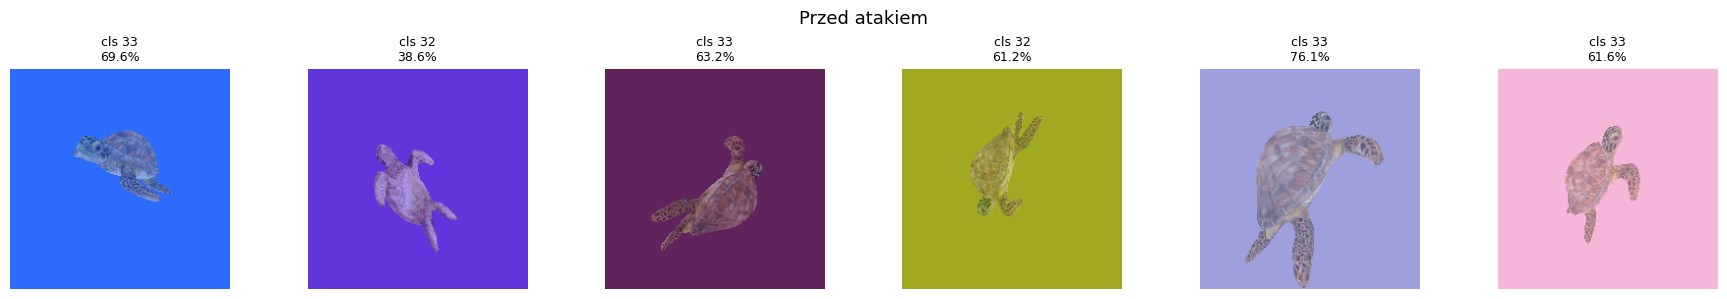
\includegraphics[width=\linewidth]{przed.png}\\[6pt]
  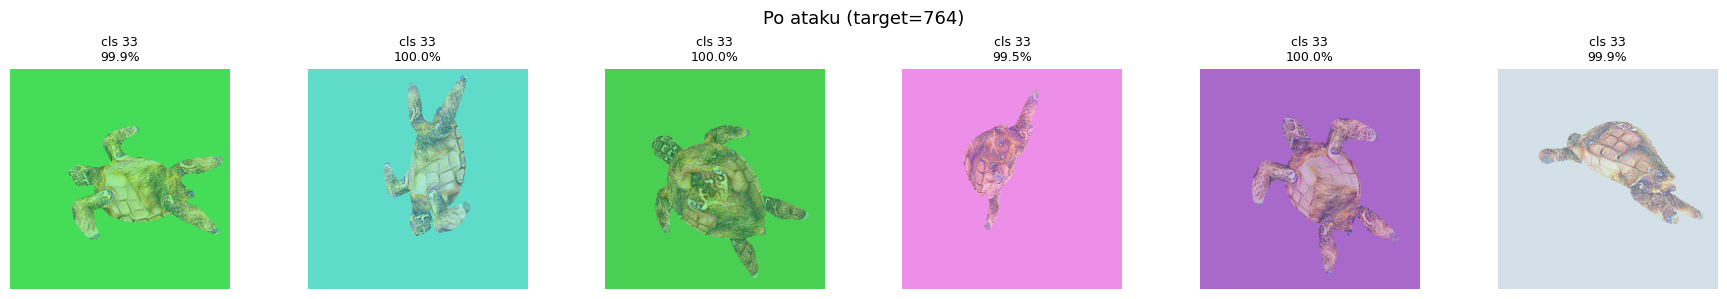
\includegraphics[width=\linewidth]{po.png}
  \caption{Top: classifier predictions \textbf{before} the attack
           (classes 32/33, confidence 38--76\%).
           Bottom: predictions \textbf{after} the attack
           (class~33, confidence 99--100\%).}
  \label{fig:results}
\end{figure}

\subsection*{What went wrong --- inverted gradient}

The classifier became \emph{more} confident about the turtle class after the attack,
rather than shifting toward rifle.
This was caused by a sign error in the gradient update:
the loss was negated before backpropagation, which reversed the direction of the update ---
instead of making the classifier more likely to predict the target class,
the texture was pushed in the opposite direction, reinforcing the original prediction.

After identifying and correcting the sign, the attack is set up properly
and a corrected run on GPU (Google Colab T4) is pending.

% ─────────────────────────────────────────────────────────────────────────────
\section{Reference}

A.\ Athalye, L.\ Engstrom, A.\ Ilyas, K.\ Kwok.
\textit{Synthesizing Robust Adversarial Examples.}
ICML 2018. \texttt{arXiv:1707.07397}

\end{document}
